\documentclass{article}
\usepackage{amsmath,amsthm,amssymb,amsfonts}
\usepackage{setspace,enumitem}
\usepackage{graphicx}
\usepackage{hyperref}
\usepackage{natbib}
\usepackage{afterpage}
\usepackage{xcolor}
\usepackage{etoolbox}
\usepackage{booktabs}
\usepackage{pdfpages}
\usepackage{multicol}
\usepackage{geometry}
\usepackage{bbm}
\usepackage{csvsimple}
\usepackage{accents}
\hypersetup{
	colorlinks,
	linkcolor={blue!90!black},
	citecolor={red!90!black},
	urlcolor={blue!90!black}
}

\newtheorem{theorem}{Theorem}
\newtheorem{assumption}{Assumption}
\newtheorem{definition}{Definition}
\newtheorem{lemma}{Lemma}
\setlength{\parindent}{0cm}
\geometry{margin = 1in}

\newcommand{\R}{\mathbb{R}}
\newcommand{\ubar}[1]{\underaccent{\bar}{#1}}
\newcommand{\F}{\mathcal{F}}
\newcommand{\xbf}{\mathbf{x}}
\newcommand{\Xbf}{\mathbf{X}}
\newcommand{\Vbf}{\mathbf{V}}
\newcommand{\zbf}{\mathbf{z}}
\newcommand{\Tbf}{\mathbf{T}}
\newcommand{\mubf}{\boldsymbol{\mu}}
\newcommand{\alphabf}{\boldsymbol{\alpha}}
\newcommand{\betabf}{\boldsymbol{\beta}}
\newcommand{\sigmabf}{\boldsymbol{\sigma}}
\newcommand{\onebf}{\mathbbm{1}}
\newcommand{\Covbf}{\text{\textbf{Cov}}}
\newcommand{\Varbf}{\text{\textbf{Var}}}

\newtoggle{extended}
\settoggle{extended}{false}

\title{ECON 899B: PS4}

\author{Alex von Hafften}

\begin{document}

\maketitle

\section*{Question 1 - Value Function Iteration}

Construct the $U_0$ and $U_1$ as the current per-period payoff vectors (do not including the T1EV shocks):

\begin{align*}
U_0 &= \alpha C \onebf(I > 1) + \lambda\onebf(I = 1)\onebf(C > 1) \\
U_1 &= \alpha C - P
\end{align*}

where $C$ is the consumption shock vector, $I$ is the inventory vector, and $P$ is the price vector across states. Following the algorithm in slide 9 of the notes on dynamic discrete choice models we use value function iteration:

\begin{align*}
EV^0 &= \log (\exp(U_0) + \exp(U_1)) + \gamma \\
EV^k &= \log (\exp(U_0 + \beta F_0 EV^{k-1}) + \exp(U_1 + \beta F_1 EV^{k-1})) + \gamma
\end{align*}

where $F_0$ is the transition matrix without investment and $F_1$ is the transition matrix with investment. 

\bigskip

The resulting $EV$ are reported in the following table:

\csvautotabular{table_1.csv}

\pagebreak

\section*{Question 2 - Policy Function Iteration}

In the table below, I compare the expected values from value function iteration ``EV" and policy function iteration based on the estimated frequencies from the simulated data ``EVhat". In addition, I include the estimated frequency based on the simulated data. I use the following algorithm from page 10 and 11 of the slides on dynamic discrete choice models:

\begin{align*}
e_0 &= \gamma - \ln \hat{P}_0\\
e_1 &= \gamma - \ln \hat{P}_1\\
P^0 &= (1 + \exp(-(\hat{P}_1 -\hat{P}_0)))^{-1}\\
F^k &= (1-P^k) .*F_0 + R^k .* F_1 \\
EV^k &= (I - \beta F^k)^{-1} ((1-P^k) .* (U_0 + e_0) + P^k .* (U_1 + e_1))\\
\tilde{V}^k &= (U_1 + \beta F_1 EV^k) - (U_0 + \beta F_0 EV^k)\\
P^{k+1} &= 1./(1 + \exp(-\tilde{V}^k))
\end{align*}

where $\hat{P}_0$ and $\hat{P}_1$ are the estimated state-level frequencies based on the simulated data and ``$.*$" and ``$./$" denotes element-by-element multiplication and division, respectively.

\bigskip

The estimates are very close.  On average, the PFI estimates are about 8 tenths of a percent off from the VFI estimates. The largest difference was just less than three percent; this was one of the two states that were constrained by the probability bounds of (0.001, 0.999). The value function iteration took 3,248 iterations and the policy function iteration only took 15 iterations.  Both were very fast, but scaling this problem up, the computational advantages of the policy function iteration could be substantial.

\pagebreak

\csvautotabular{table_2.csv}

\pagebreak

\section*{Question 3 and 4 - Maximum Likelihood Estimation}

The log-likelihood function is:

\begin{align*}
\sum_i & a_i \ln P(s_i) + (1-a_i) \ln (1 - P(s_i)) \\
\text{s.t. } & P(x_i) = \Psi(x_i)
\end{align*}

where $\Psi(\cdot)$ is the contraction mapping laid out in question 2.

\bigskip

I used Brent's method to find the MLE estimate of $-4.020022$ for $\lambda$.  A figure of the log-likelihood over values for $\lambda$ is below:

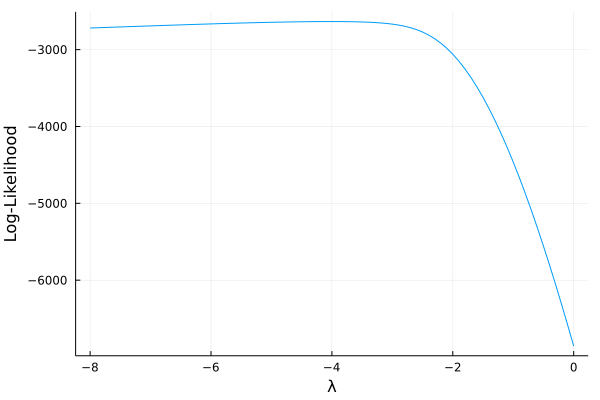
\includegraphics[scale=.75]{question_4.png}

\end{document}

